\documentclass{article}
\usepackage[utf8]{inputenc}
\usepackage{tikz,graphicx,hyperref,amsmath,amsfonts,amscd,amssymb,bm,cite,epsfig,epsf,url}

\title{lecture 5:spark  }
\author{wbg231 }
\date{January 2023}

\begin{document}

\maketitle

\section{review}
\begin{itemize}
\item name node manages meta data, coordinates data access and ensures data integrity 
\item the data note stores each block of data and does data processing could be where computation is done in map reduce 
\item think of it as worker and head node 
\subsection*{why spark}
\item what was good about map reduce
\begin{itemize}
    \item it is scalable on hadoop and allows for parallel processing of big data
    \item it has fault tolerance 
    \item it works well with off the shelf hardware 
    \item takes care of most of the really gritty stuff of parallel computing like job scheduling 
\end{itemize}
\item what was bad about map reduce
\begin{itemize}
    \item it is build on an acyclic data flow models
    \item it is to low level
\end{itemize}
\subsection*{why is it to low level}
\begin{itemize}
    \item map reduce is great for one time jobs with simple dependencies on big data
    \item but it can not work with iterative jobs, complex queries exc  
\end{itemize}
\subsection*{gradient descent example}
\item imagine trying to do gradient descent in map reduce 
\item  as you can see here 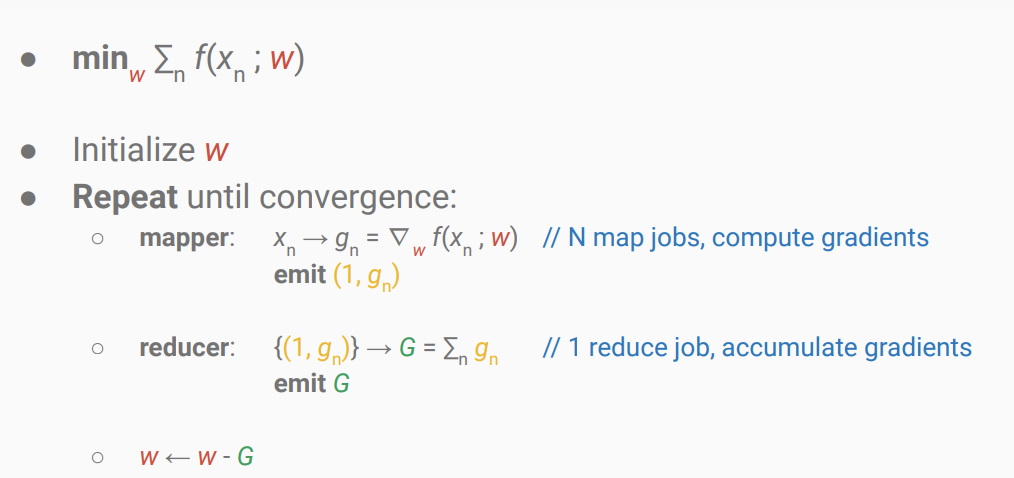
\includegraphics{images/Screenshot 2023-05-10 at 1.03.43 AM.png}
\item you would have to at every stage in the loop map n jobs to compute the gradient 
\item and then reduce those into one value by taking a sum adn use that to take a step 
\item so each step of a gradient descent algorithm requires a full map reduce 
\item and we do note about the previous iteration once it is done (so they could be parallelized)
\item further notice that the reducer can not start it's job until all the mappers are done with theres so there is high latency
\item more generally some computations have complex pipelines that are ill suited for map reduce 
\item like for instance in cases where we want to do many iterations quickly
\subsection*{Resilient distributed records}
\item Resilient distributed records or RDD's are one solution to this
\subsection*{reusing data}
\item complex computations usually have intermediate steps 
\item map reduce only likes to compute something save an intermediate result and move onto the next step
\item tht can be wasteful and awkward ot use for some problems 
\subsection*{RDDs}
\item an RDD has
\begin{itemize}
    \item a data source 
    \item a lineage graph of transformations to apply to the data 
    \item interfaces for data partitioning and iteration
\end{itemize}
\item think of this as deferred computation
\begin{itemize}
    \item nothing is computed until you ask for for it 
    \item nothing is saved until you say so 
    \item this makes optimization easier
\end{itemize}
\item we are going to say RDD[T] is an RDD with type t 
\subsection*{RDD example: log processing}
\item suppose we have a long document and we want to find all the lines in that document that start with the word error 
\item \includegraphics*[width=10cm]{images/Screenshot 2023-05-10 at 1.19.52 AM.png}
\item so first off note what the colors mean \textcolor{yellow}{rdd} \textcolor{blue}{data} \textcolor{red}{transformations} \textcolor{green}{action}
\item so the first thing we do is read the file into an rdd 
\item then we transform the data using two filters and a map 
\item then we take an action and collect the data
\item note that no computation happens until the action (in this case collect)
\subsection*{transformations}
\item transformations turn one or more rdds into a new rdd 
\item transformations are cheap to construct because they do not actually do the computation until and action is taken 
\item building an rdd is like writing a map reduce script or sql query (nothing goes until you click enter)
\item example transformations are map, filter, union 
\subsection*{actions}
\item actions are what execute the computation defined by an RDD
\item results of actions are not RDDs
\item example actions: count, collect, reduce, save
\subsection*{work backwards then forwards}
\item notice that every step depends on what happened before it 
\item and previously computed Rdd's can be cached and reused 
\item any lost/corrupted RDD can be rebuilt from a linear graph 
\subsubsection*{lineage graph }
\item a linear graph does not have to be a line there can be any rdd can have multiple parents 
\item once a parent rdd is computer it can be cached and used by many descents
\item lineage can be pipelined 
\item we do not need to wait for all lines to finish to build errors 
\item there is no need for intermediate storage like in map reduce 
\item more or less until an action is taken we have the linage graph so any worker node can do all transformations in it's lineage graph as soon as it finishes one with out weighting for the others to finish 
\item compare this to non pipelined implementations that have to finish all of one transformation then move to the next.
\subsection*{slido}
\item RDDs can depend on each other only in a feed forward one to one fashion 
\item i think false, there can be multiple parents so it does not have to be one to one 
\subsection*{the rdd interface}
\item partitions() returns a list of partitions kinda like splits in map reduced 
\item preferred locations (p) ie the HDFS node where partition p can be found
\item dependencies() the the dependencies for this RDD
\item iterator(p, parentitters) get elements of partition p given parents partitions
\item partitioner  get meta data about how the rdd  is partitioned
\subsection*{narrow and wide dependencies}
\item narrow dependencies all the partitions of one RDD go to one child rdd 
\item this is good we have low computation, data stays localized, it is easy to pipeline, it is easy to recover from computer failure
\item a wide dependencies is when the partitions of parent RDD goes to multiple child RDD partitions
\item high computation
\item high latency
\item hard to pipeline 
\item hard to recover data if a computer fails
\subsection*{slido}
\item much like in map reduce spark ahs to wait for a step in a lineage to complete 
\item false that is the whole point 
\section*{actually using spark in 2023}
\subsection*{V0 in  2009-2012}
\item a cluster computing frame work for using RDDs
\item integrates with hadoop ecosystem 
\item written in scala with API in other languages like R java and python
\subsection*{architecture: session and driver}
\item the driver is the process that you run on the head or login node 
\item the session object connects your code to the cluster and compute nodes. 
\subsection*{why is spark written in scala}
\item RDD design fits well with functional programming
\item scala compiles to the java virtual machine, which is compatible with python
\subsection*{closure}
\item closure are a functional programming concept that combines a function with its environment 
\item scala is well suited for this 
\subsection*{gradient descents in spark}
\item here is the psudo code 
\item as we can see the outer loop still runs in series 
\item but the inner loop can run in paralell 
\item so there is a lot less waiting than if the inner loop had to wait for every othe rpoint evert time 
\item then the grad is a shared accumulator which is a write only data structure that always is added to 
\subsection*{beyond scala}
\item spark can work in a lot of languages now 
\item beware r and python spark still may not be as fast as scala spark
\item it is expensive to use operations that are just in python since but spark tries to limit this by seralizing all data
\item so we do not write raw rdd code in python, but we do use existing packages written in scala with python bindings 
\section*{spark data frames }
\item rdds are very good but can be cumbersome, for ad hoc computations
\item data frames are common representions in many languages
\item spark 2 has a data frame api as a primary interface
\subsection*{rdd are more than columns}
\item RDDs can be derived from other Rdds through transformations
\item RDD also have partition information which influinces how they are stored in HDFS
\item one or more RDDs can be used to form a data frame 
\item could have an RDD with compound types but RDDs are more convient 
\subsection*{data frames and rdds }
\item data frames in spark are like relations in RDBMS 
\item they have well defined shcmes with types over columns 
\item each row is pretty much a tuple
\item data frame operations are translated into RDD transformations
\item RDD transfomration can be executed within theJVM, that means while using a data frame we can use python or other language operations with out seralization 
\item when using RDBMS we often think of our data in rows 
\item data frames are implemented as a collection rdd with 1 column = 1 rdd 
\item that is data frames are column oriented 
\item this does not change how we interact with them much as a programer but does change how we think about storage of data 
\subsection*{spark sql}
\item we cab also use sql queries in spakr (or us a data frame object oriented method)
\item queries are executable against data frames 
\item data frames are secretly RDDs not RDBMS
\item queries can be optimized by analyzing the lineage graph of the RDD that is being worked with 
\subsection*{reparitioning}
\item before running an action on a dataframe run teh explain method 
\item this will tell you an execution plan, and might help identify bugs
\item be carefull with .collect() it can be a bad includegraphics
\subsection*{map reduce requires both map and reduce to be deterministic, is this the same for map reduce}
\item true for map reduce and for spark
\subsection*{determinism in spark}
\item transfomrations in spark need have to be deterministic
\item with out this reconstructin from a lineage graph would not make sense 
\item what problems could this present when would ramdomization be helpful
\subsection*{slido}
\item do any of the stonebreaker critisms of map reduce apply to spark? 
\item it is higher level so that is good 
\item it has query optimization but that does not replace indexing 
\item it is missing RDMS features, but partitioning is kinda liek that, we do have shcemas transactions matter les due to read only data 
\item RDMS compatable speark i not a RDMS ut it is better integrated with data frames
\subsection*{wrap up on spark}
\item RDD frame work is more flexible than map reduce
\item chacing can make interactive job faster 
\item spark sql dta frames make devlopment faster 

\end{itemize} 
\end{document}
